\documentclass[11pt, a4paper]{article}

% --- Packages ---
\usepackage[utf8]{inputenc}
\usepackage[margin=1in]{geometry} % Standard professional margins
\usepackage{graphicx}             % For importing UML diagrams (PNG, PDF, JPEG)
\usepackage{booktabs}             % For high-quality professional tables
\usepackage{tabularx}             % For tables that auto-stretch to page width
\usepackage[table,xcdraw]{xcolor}
\usepackage{array}
\usepackage{hyperref}             % Makes the Table of Contents clickable
\usepackage{enumitem}             % For lists
\hypersetup{
    colorlinks=true,
    linkcolor=blue,
    filecolor=magenta,
    urlcolor=cyan,
    pdftitle={AstraLog-HPC Phase 1},
}

% Ensure the TOC shows up to 3 levels (Section, Subsection, Subsubsection)
\setcounter{tocdepth}{3}

\begin{document}

% ==========================================
% FRONT PAGE (As required by Section 4)
% ==========================================
\begin{titlepage}
    \centering
    \vspace*{2cm}

    {\scshape\LARGE Politecnico di Milano \par}
    \vspace{1cm}
    {\scshape\Large Software Engineering for HPC\par}
    \vspace{1.5cm}

    \hrule
    \vspace{0.5cm}
    {\huge\bfseries AstraLog-HPC \\ \vspace{0.3cm} \Large Requirement Analysis and Design Document \par}
    \vspace{0.5cm}
    \hrule

    \vspace{2cm}

    {\Large\itshape
    Domenico De Giorgio - 10854350 \\
    Leonardo Pelorosso - 10779110 \par}

    \vfill

    {\large \textbf{Version:} 1.3.2 \par}
    {\large \textbf{Release Date:} \today \par}
    {\large \textbf{Academic Year:} 2025-2026 \par}
\end{titlepage}

% ==========================================
% TABLE OF CONTENTS
% ==========================================
\newpage
\tableofcontents
\newpage

% ==========================================
% 1. THE PROJECT AND PROJECT GOALS
% ==========================================

\section{The project and project goals}

\subsection*{Overview}
Modern space missions rely on a continuous and massive flow of telemetry data from various onboard subsystems. Ensuring the safety and operational integrity of a spacecraft is a mission-critical task that requires the ability to process this data efficiently and detect potential failures or deviations in real-time.

\subsection*{The Problem}
The data transmitted from space is often high-volume and subject to corruption or noise due to the harsh nature of long-distance communication. Furthermore, identifying an anomaly is rarely a matter of checking a single value; it requires analyzing complex relationships between different sensors and tracking how data evolves over time. Without an automated, high-performance system, mission operators risk missing critical warning signs that could lead to system failure.

\subsection*{Project Objectives}
The primary goal of this project is to develop a high-performance software solution dedicated to spacecraft health monitoring and anomaly detection. The system is designed to:

\begin{itemize}
    \item \textbf{Ensure Data Integrity:} Automatically filter and validate incoming telemetry streams to eliminate corrupted or malformed data before it reaches the analysis stage.
    \item \textbf{Automate Anomaly Detection:} Implement a flexible monitoring engine capable of evaluating sensor behavior against complex operational logic and cross-sensor correlations.
    \item \textbf{Streamline Reporting:} Provide a clear distinction between nominal system states and anomalous events, ensuring that valid data is preserved for analysis while critical alarms are immediately flagged.
    \item \textbf{Achieve Scalability:} Optimize the system for High-Performance Computing (HPC) environments to handle the computational load of modern, data-intensive space missions.
\end{itemize}

\subsection*{Final Goal}
The ultimate success of the project lies in providing a robust, scalable architecture that transforms raw, noisy telemetry into actionable insights, ensuring the long-term safety and reliability of complex aerospace systems.

\newpage
% ==========================================
% 2. REQUIREMENT ANALYSIS
% ==========================================
\section{Requirement analysis}

\subsection{Relevant human and non-human actors}
\subsubsection{Human actors}
\begin{description}[align=left, leftmargin=2cm]
    \item[\textbf{System Operator:}] Configures and initializes the system via Command Line Interface (CLI) by providing five mandatory arguments: \texttt{--batch\_size}, \texttt{--input\_path}, \texttt{--output\_path}, \texttt{--rules\_path}, and \texttt{--sensors\_path}. After the automated execution, the operator consumes the resulting output files generated at the specified paths (e.g., \texttt{valid\_data.csv} and \texttt{alarms.log}).
\end{description}

\subsubsection{Non-Human actors}
\begin{description}[align=left, leftmargin=2cm]
    \item[\textbf{Spacecraft Master System:}] Produces a continuous stream of JSON packets containing data from sensors measurements.
    \item[\textbf{SLURM Job Scheduler:}] The external workload manager operating on the Galileo 100 cluster. It is responsible for queuing the batch job, allocating the requested compute resources (CPU/RAM), and automatically triggering the execution of the AstraLog-HPC containerized application without user intervention.
\end{description}

\subsection{Use cases}


\subsubsection{Overview and Diagram}
The AstraLog-HPC system is designed to operate autonomously within an HPC environment, interacting with telemetry streams and configuration files. The following use cases describe the functional scope of the system.

% Placeholder per il diagramma
\begin{figure}[h]
    \centering
    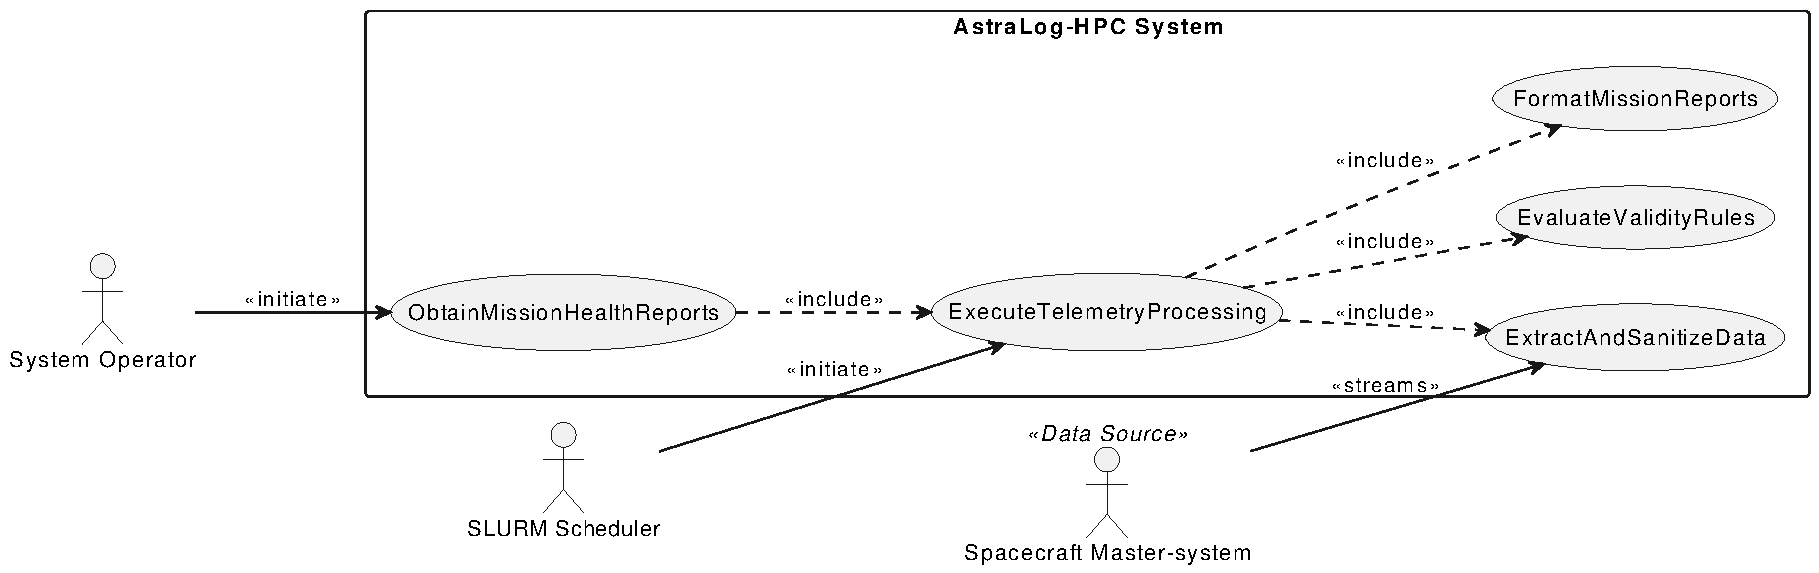
\includegraphics[width=1\textwidth]{diagrams/use_case_diagram.pdf}
    \caption{AstraLog-HPC Use Case Diagram showing the interaction between the telemetry stream, the rules engine, and the output logging system.}
\end{figure}

\noindent

The system identifies five primary use cases:
\begin{enumerate}[label=\textbf{UC-\arabic*}, align=left, leftmargin=2cm]
    \item \textbf{ObtainMissionHealthReports:} It starts when the System Operator needs to verify the spacecraft's status, configures the environment, and schedules the job through the SLURM scheduler; it ends when the Operator successfully retrieves the final output files.

    \item \textbf{ExecuteTelemetryProcessing:} It starts when the SLURM Scheduler allocates the requested HPC resources and boots the containerized execution; it ends when the entire input dataset has been processed and the output streams are closed.

    \item \textbf{ExtractAndSanitizeData:} It starts when the Spacecraft Master-system sends a new chunk of data to the system; it ends when a safe batch of raw strings is loaded and sanitized into a structured memory format.

    \item \textbf{EvaluateValidityRules:} It starts when a sanitized batch of telemetry is passed to the rules engine; it ends when all the rules are evaluated via vectorized operations, separating anomalous timestamps from nominal ones and the results are saved in temporary memory.

    \item \textbf{FormatMissionReports:} It starts when the evaluation phase produces the lists of valid and anomalous records; it ends when the system deterministically formats and appends the outputs to either \texttt{valid\_data.csv} or \texttt{alarms.log}.
\end{enumerate}

\subsubsection{Detailed Use Case: EvaluateValidityRules}
The most critical use case is \textbf{UC-4}, as it process ensures the accurate identification of nominal data and errors.

\begin{table}[h]
\centering
\renewcommand{\arraystretch}{1.5}
\begin{tabular}{|p{3.5cm}|p{10.5cm}|}
\hline
\textbf{Use Case Name} & EvaluateValidityRules (UC-4) \\ \hline
\textbf{Actors} & AstraLog-HPC System (Rules Engine), System Operator\\ \hline
\textbf{Description} & The system evaluates a batch of sanitized telemetry data. For each timestamp, it checks if any validity rule is triggered. \\ \hline
\textbf{Pre-conditions} &
\texttt{rules.json} valid for Rules Engine initialization. \newline
A batch of extracted and sanitized sensor data.
\\ \hline
\textbf{Trigger} & Extract\&SanitizeData outputs a preprocessed batch.
\\ \hline
\textbf{Main Success Scenario (Main Flow)} &
1. Iterates through the rules present in the \texttt{rules.json} by priority, acting on the batch entries that contain the same sensor\_id as the rule. \newline
2. The Rules Engine evaluates Simple, Step and Stateful rules, and at last it evaluates Correlation rules. \newline
3a. If the telemetry readings from all sensors for a given timestamps are valid, they get appended in the valid\_telemetry temporary variable. \newline
3b. If a timestamp has one or more invalid readings, those readings get appended in alarm\_telemetry temporary variable. \newline
4. Both variables are passed on to the OutputFormatter.
\\ \hline
\textbf{Alternative Flows} &
\textbf{A1. Data Insufficiency for Stateful/Step Rules:} If the previous timestamp ($T_{n-1}$) is missing, the system skips evaluation for relative rules and logs a warning.
\\ \hline
\textbf{Post-conditions} &
\texttt{valid\_telemetry} temporary variable contains only valid data in the analyzed batch. \newline
\texttt{alarm\_telemetry} temporary variable contains a complete trace of all detected anomalies in the analyzed batch.
\\ \hline
\end{tabular}
\end{table}
\newpage
\subsection{Domain Assumptions}

To maintain consistency between the long-term requirements of the system (Target Architecture) and the current software increment (Current Scope), the Domain Assumptions have been redefined using an incremental approach. This allows the validation of the processing logic through offline CSV files, while preserving the architectural vision of the future continuous JSON stream.

\begin{enumerate}[label=\textbf{DA-\arabic*:}, align=left, leftmargin=2cm]
    \item \textbf{System Evolution \& Ingestion Scope:} The target architecture of the system expects the ingestion to occur via a continuous stream of JSON packets from each sensor for the whole duration of the mission. However, within the current implementation milestone (\textit{Current Scope}), the system handles the offline, batch-based ingestion of historical or simulated data stored in CSV text files.

    \item \textbf{Sensor Specifications:} Sensors can be of any type specified in the \texttt{sensors.yaml} file, and there can be multiple sensors of the same type, each producing its own measurement identified by a unique \texttt{sensor\_id}. This principle applies identically to both the current CSV format and the future JSON stream.

    \item \textbf{Temporal Constraints \& Emulated Streaming:} In the complete target system, at each fixed timestamp, all sensors produce a measurement wrapped in a JSON packet. In the current phase, this temporal sequentiality is preserved within the CSV file; the system adopts a chunk-based reading mechanism (\textit{batched reading} via \texttt{pl.read\_csv\_batched}) to emulate the high-performance, stream-oriented processing of the target architecture.

    \item \textbf{Data Delivery and Retention:} It is assumed that all telemetry packets generated for the current mission have been successfully recorded and persisted into the input CSV file, assuming no data loss occurs prior to the batch processing. In the target system, this translates to assuming that all produced JSON packets successfully arrive at their destination.

    \item \textbf{Data Corruption \& Robustness:} At each timestamp, any number of records in the CSV file can be corrupted or anomalous. In strict analogy to the target system (which mandates rejecting corrupted JSONs), the current \texttt{CSVTelemetryReader} component must identify and handle three macro-categories of errors:
    \begin{itemize}[leftmargin=0.5cm]
        \item \textbf{Malformed Data/CSV:} Truncated lines, missing delimiters, quoting issues, or violations of the RFC 4180 standard (corresponding to \textit{Malformed JSON} syntax).
        \item \textbf{Schema Errors:} Record or CSV rows missing mandatory fields (\texttt{time\_stamp}, \texttt{sensor\_id}, \texttt{value}, \texttt{priority}), meaning missing columns or unallowed null values.
        \item \textbf{Type Errors:} Invalid data types present in the columns (e.g., text strings that cannot be parsed into the expected numerical or temporal types).
    \end{itemize}

    \item \textbf{Rule-Based Validation:} Each measurement (whether extracted from the current CSV batch or the future JSON stream) can be subject to none or any number of validity rules specified in the \texttt{rules.json} file.

    \item \textbf{Validity Rule Types:} Validity rules are fixed for the whole duration of the mission and can be ONLY of one of the following 4 types:
    \begin{itemize}[leftmargin=0.5cm]
        \item \textbf{Simple Rule / Absolute Threshold:} Checks if a value exceeds a fixed threshold at a given time.
        \item \textbf{Step Difference Rule / Relative Variation:} Checks the difference between the current measurement and the measurement at the previous \texttt{time\_stamp}.
        \item \textbf{Stateful Rule / Measurement Persistence:} An anomaly is triggered only if a specific simple condition persists uninterrupted for a given number of consecutive \texttt{time\_stamps}.
        \item \textbf{Logical Correlation Rule:} Combines the Boolean outcomes of other evaluated rules at the same timestamp using standard logical operators (AND / OR).
    \end{itemize}

    \item \textbf{Rule Identification:} Each validity rule has a unique \texttt{rule\_id} to ensure traceability during the evaluation process across all ingested data formats.

    \item \textbf{Rule Priority and Execution:} Each validity rule has a priority level (low, medium, high) which applies within a single rule type and implies that rules with higher priority are evaluated before lower priority ones.
\end{enumerate}

\subsection{Requirements}

\subsubsection{Functional requirements}
\begin{enumerate}[label=\textbf{FR-\arabic*:}, align=left, leftmargin=2cm]
    \item the system shall read the sensor configuration from the local \texttt{sensors.yaml}.
    \item the system shall allow jobs to be scheduled with a batch\_size through command line argument.
    \item the system shall read a local \texttt{rules.json} file specifying rules of data validity.
    \item system shall receive a stream of data in form of JSON packets.
    \item system shall filter data packets checking their integrity and temporarily buffer the valid records in memory (RAM) prior to evaluation, without writing intermediate temporary files to disk.
    \item when size of batch\_file reaches a threshold value specified in batch\_size, system shall apply validity rules to buffered data, respecting per-type priority ordering.
    \item if ALL data in analyzed time\_stamp are valid (NO rule violated), system shall append them to valid\_data.csv.
    \item if one or more data in analyzed time\_stamp are NOT valid, system shall enter an anomalous state and NOT save that time\_stamp in valid\_data.csv and append warnings to alarms.log file.
    \item in the event of a critical execution failure, the system shall produce and store an ERROR message for future diagnosis.
\end{enumerate}
\subsubsection{Non-functional requirements}
\begin{enumerate}[label=\textbf{NFR-\arabic*:}, align=left, leftmargin=2cm]
    \item system shall avoid any modification to the files that implies changing already saved information, only allowing appending operations.
    \item system shall prioritize availability and correctness.
    \item system shall process continuous data stream without data loss.
    \item in the event of an abnormal termination the system shall maintain the most recent valid version of valid\_data.csv and alarms.log.
\end{enumerate}
\subsubsection{Constraints requirements}
\begin{enumerate}[label=\textbf{CR-\arabic*:}, align=left, leftmargin=2cm]
    \item system shall be implemented either in C++ or Python.
    \item system shall accept input files with the following specified format:
    \begin{itemize}[leftmargin=0cm]
        \item a file containing input packets:
        \begin{verbatim}
        {
            "timestamp": [ISO 8601],
            "sensor_id": [str],
            "value": [float],
            "priority": [LOW/MEDIUM/HIGH],
        }
        \end{verbatim}
        \item \textbf{\texttt{rules.json:}}
        \begin{verbatim}
        {
            "rule_id": [str],
            "type": [simple/step_difference/stateful/correlation],
            "sensor_id": [str],
            "operator": [math_symbol],
            "value": [float],
            "consecutive_measurements": [int], #for stateful type only
            "conditions": [ruled_id_1, ...], #for correlation type only
            "priority": [LOW/MEDIUM/HIGH],
        }
        \end{verbatim}
        \item \textbf{\texttt{sensors.yaml:}}
        \begin{verbatim}
        {
            sensors:
            - id: [str]
              sampling_rate: [int]Hz
              unit: [str]
            - ...
        }
        \end{verbatim}
    \end{itemize}
    \item system shall produce output files with the following specified format:
    \begin{itemize}[leftmargin=0cm]
        \item \textbf{\texttt{valid\_data.csv:}}\newline TIMESTAMP; NOMINAL; [SENSOR\_1]:[VALUE\_1]\textbar[SENSOR\_2]:[VALUE\_2]\textbar\dots
        \item \textbf{\texttt{alarms.log:}}\newline TIMESTAMP; RULE\_ID; PRIORITY; VIOLATED\_SENSOR(S); CURRENT\_VALUE(S) \par \textit{(Note: For correlation rules, list all sensors and values involved in the parent rules).}
    \end{itemize}
\end{enumerate}
\newpage

% ==========================================
% 3. DESIGN
% ==========================================
\section{Design}

\subsection{General description of the architecture}
The AstraLog-HPC architecture is a highly modular, decoupled pipeline optimized for unattended batch processing in an HPC environment (SLURM). Based on SOLID principles, it comprises five distinct components interacting exclusively via standardized interfaces (Figure \ref{fig:component_diagram}).

\begin{figure}[htbp]
    \centering
    % Change the filename below to match exactly what you uploaded to Overleaf
    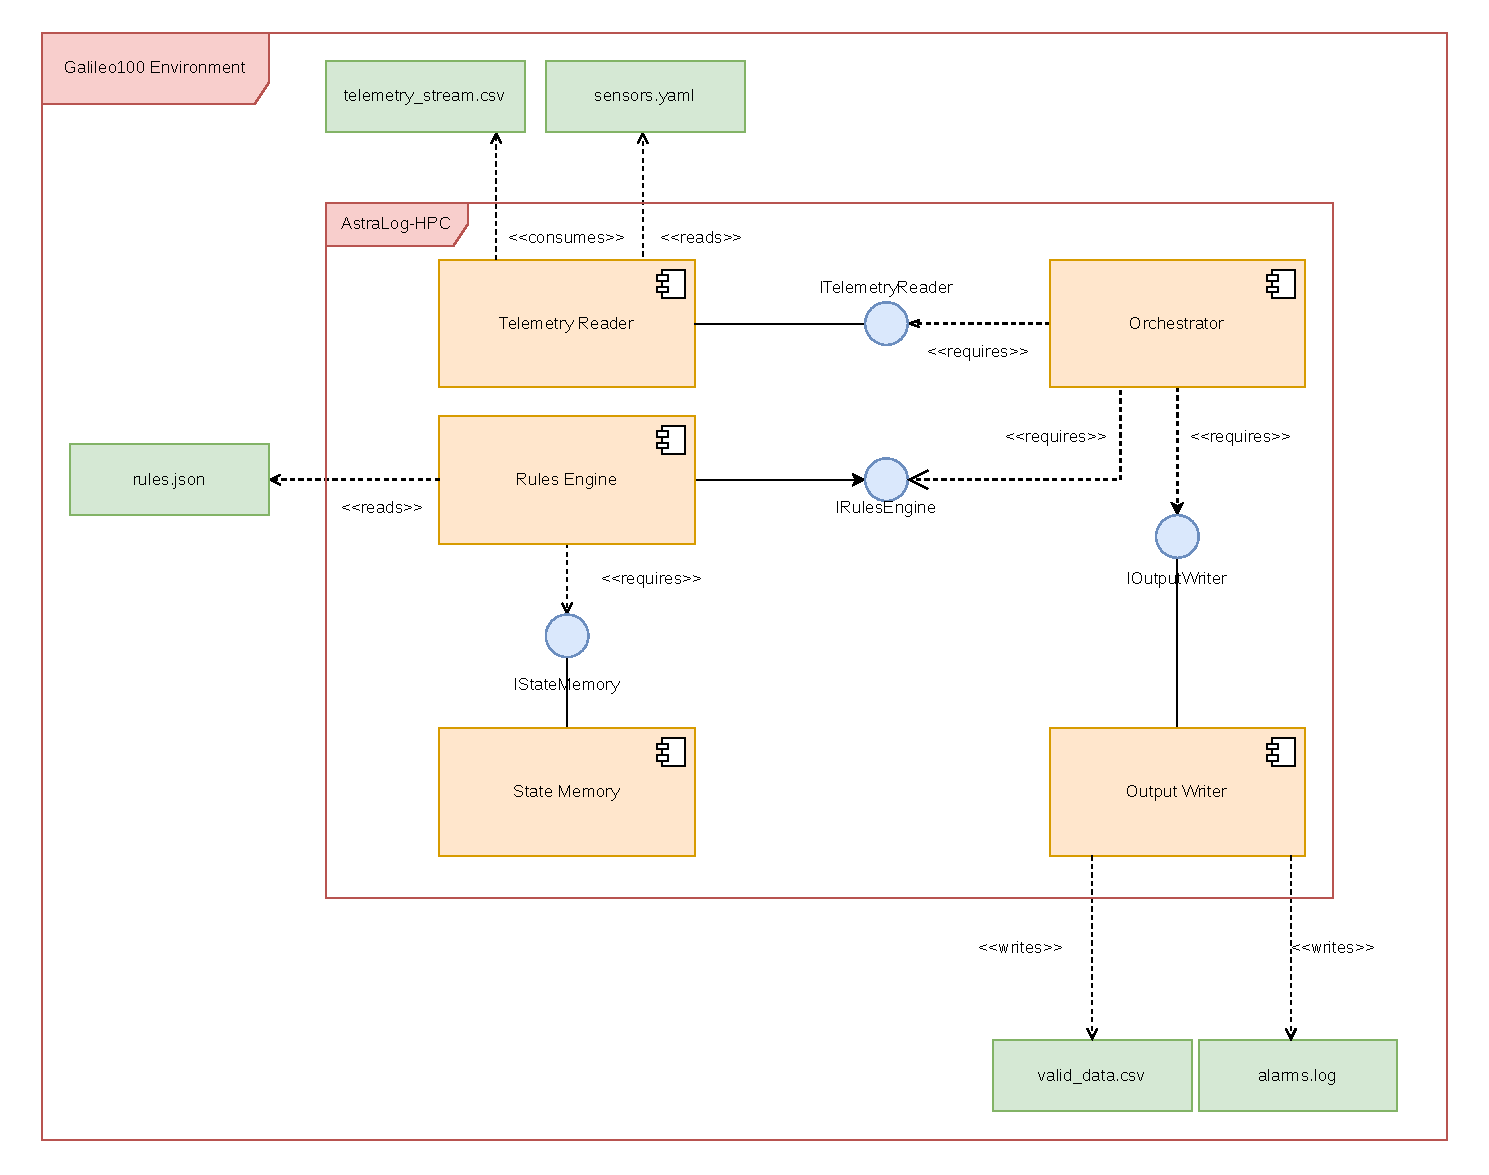
\includegraphics[width=\textwidth]{diagrams/component_diagram.pdf}
    \caption{Component Diagram of the AstraLog-HPC application.}
    \label{fig:component_diagram}
\end{figure}

A central orchestrator automates data ingestion, rule evaluation, and output generation. The core components are:

\begin{itemize}
    \item \textbf{Telemetry Ingestor:} Consumes \texttt{telemetry\_stream.csv} and reads \texttt{sensors.yaml}. It parses the payloads, discards malformed packets, and supplies clean data via the \newline \texttt{ITelemetryReader} interface (concrete implementation: \texttt{CSVTelemetryReader}).

    \item \textbf{Batch Orchestrator:} The primary controller. It uses the \newline \texttt{ITelemetryReader} interface to accumulate telemetry into in-memory batches, triggering the evaluation phase once the configured size is reached.

    \item \textbf{Rule Engine:} Exposes the \texttt{IRulesEngine} interface (concrete implementation: \newline \texttt{PolarsRulesEngine}). It reads \texttt{rules.json} to apply the four prioritized rule types (Simple, Step, Stateful, Correlation) to the batch.

    \item \textbf{State Memory:} Exposes the \texttt{IStateMemory} interface (concrete implementation: \newline \texttt{DictStateMemory}). It acts as an in-memory cache to store previous sensor states required by the Step Difference and Stateful rules.

    \item \textbf{Output Writer:} Implements the \texttt{IOutputWriter} interface (concrete implementation: \texttt{CSVOutputWriter}). It securely appends nominal timestamp data to \texttt{valid\_data.csv} and logs all constraint violations to \texttt{alarms.log}.
\end{itemize}

\subsection{Sequence diagrams}

To illustrate the dynamic behavior of the system, two distinct execution paths are provided. Figure \ref{fig:seq_nominal} demonstrates the nominal processing of a batch evaluating Simple Rules, while Figure \ref{fig:seq_stateful} illustrates the complex interaction required to evaluate a Stateful Rule over consecutive measurements.

\begin{figure}[htbp]
    \centering
    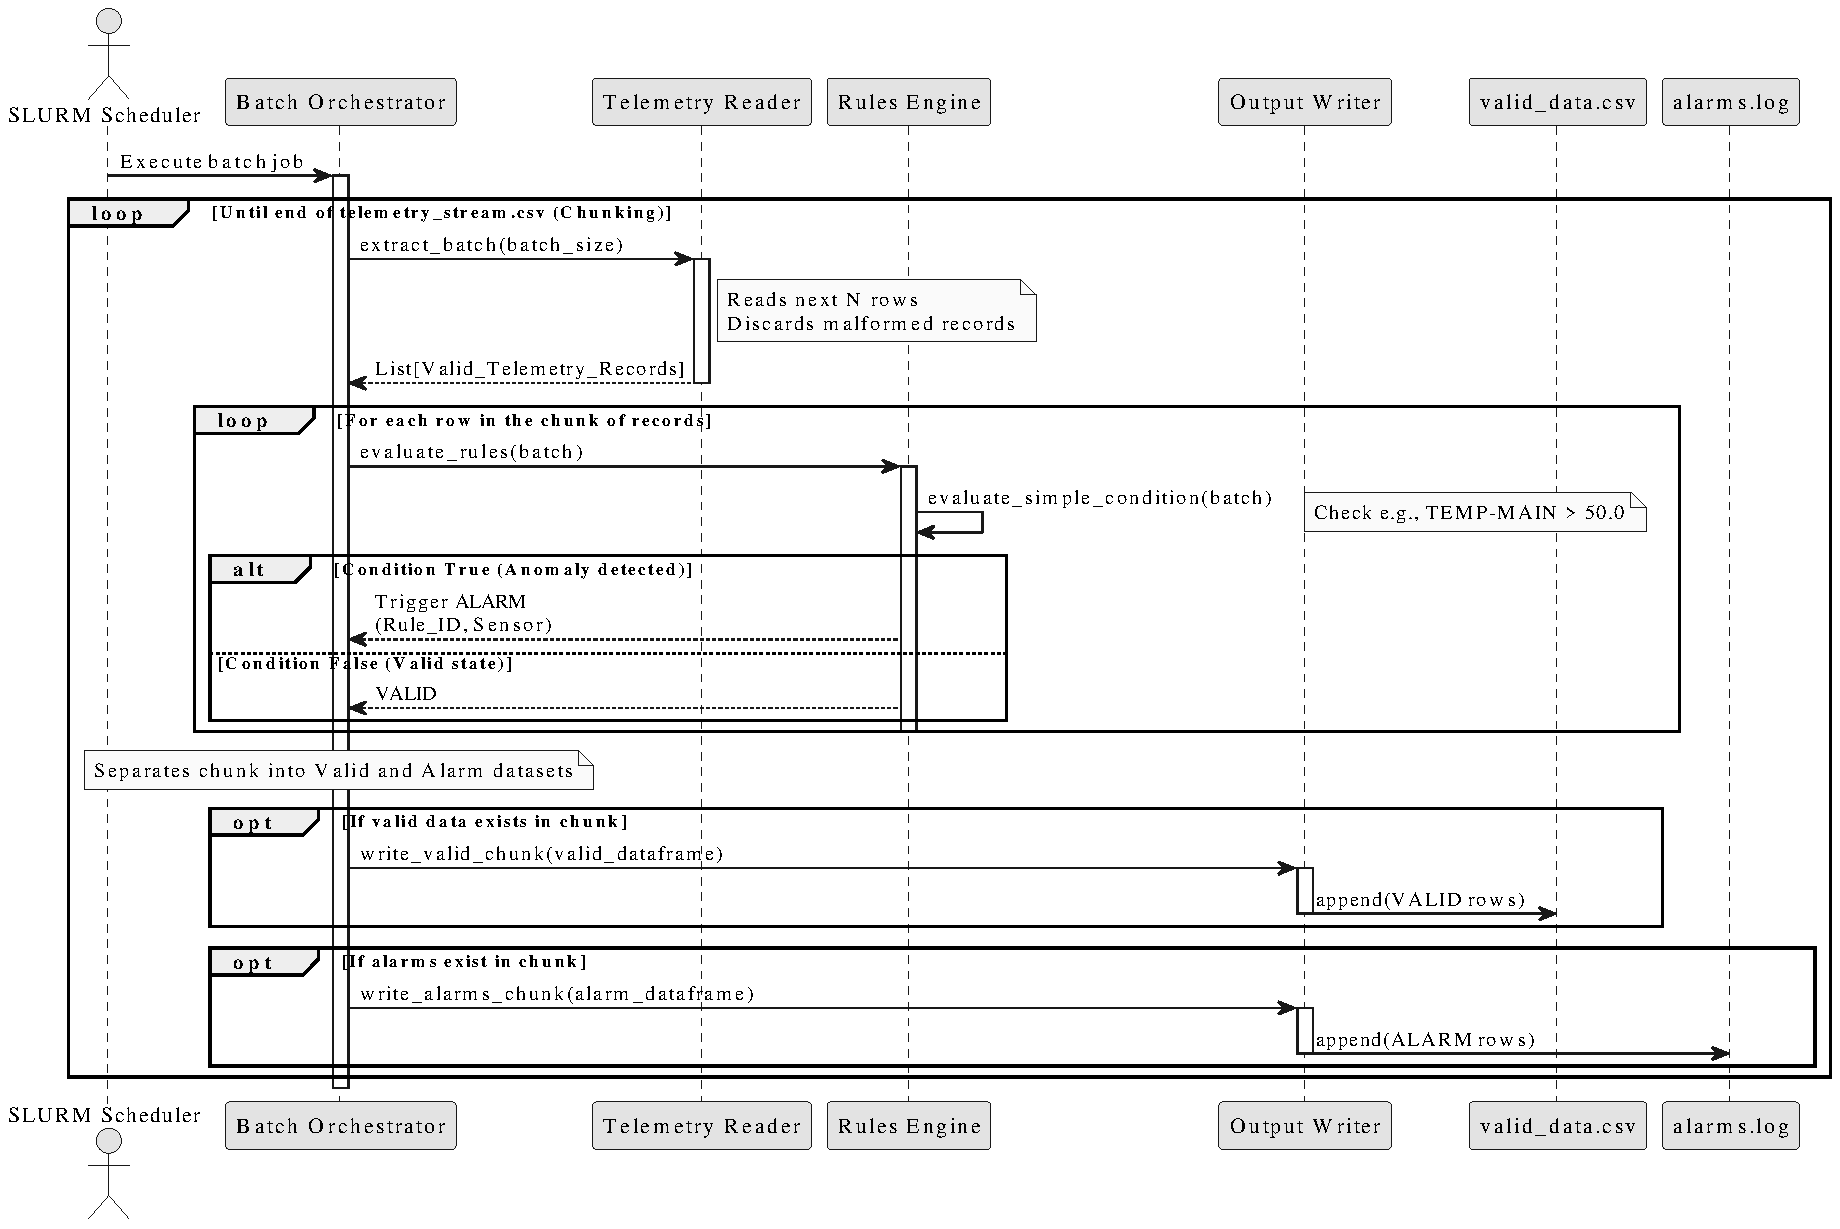
\includegraphics[width=\textwidth]{diagrams/sequence_simple.pdf}
    \caption{Sequence Diagram showing the nominal evaluation of a Simple Rule.}
    \label{fig:seq_nominal}
\end{figure}

\begin{figure}[htbp]
    \centering
    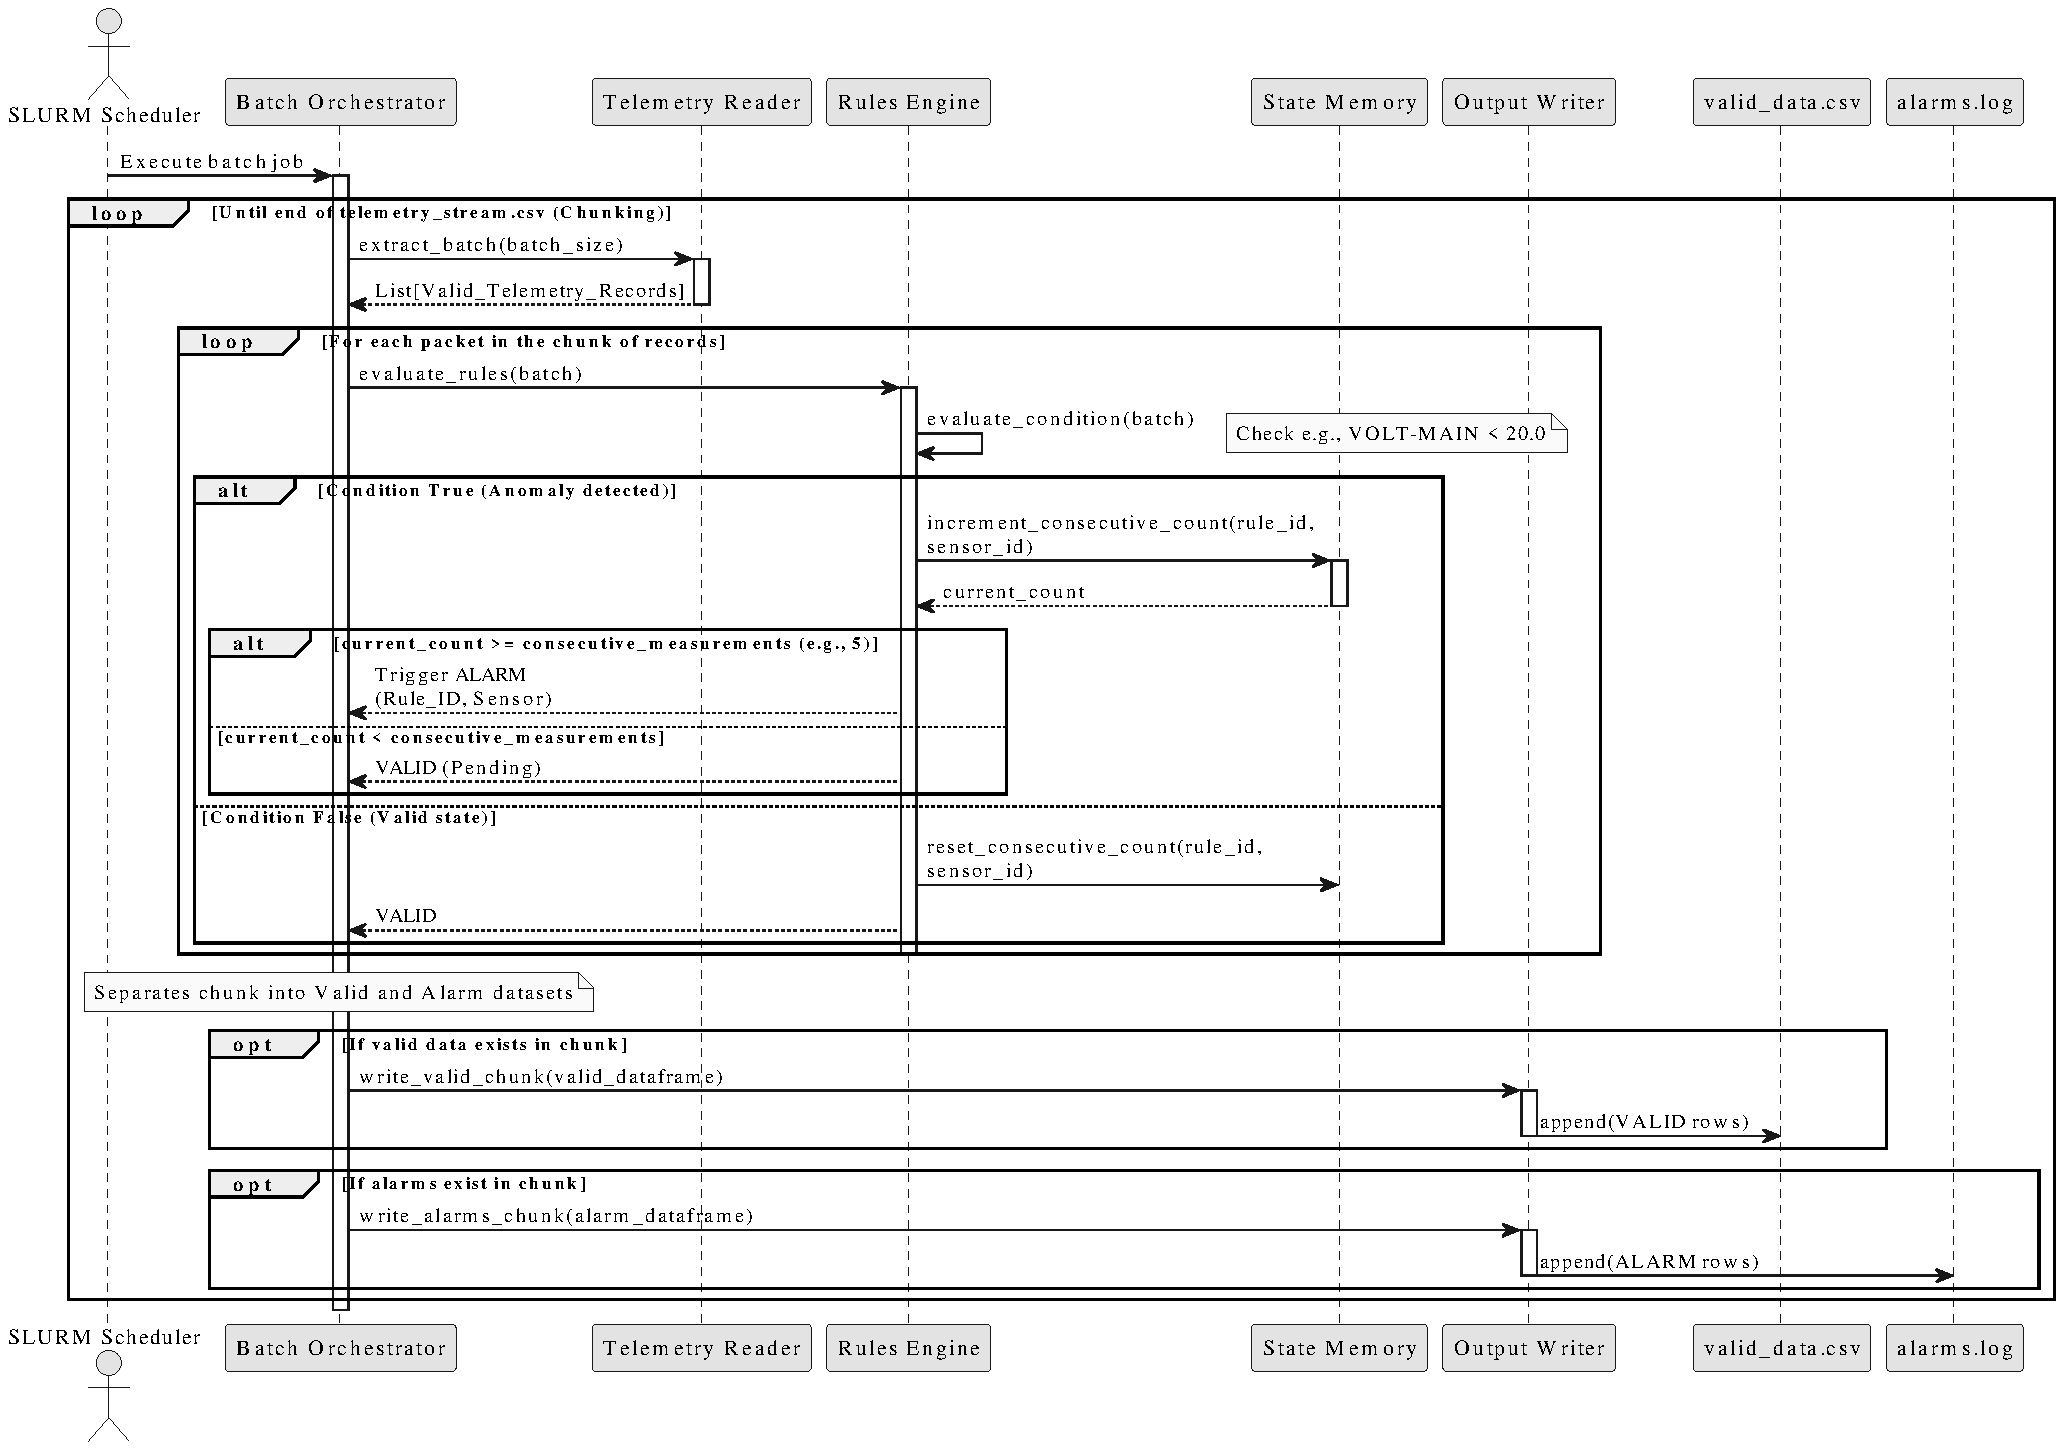
\includegraphics[width=\textwidth]{diagrams/sequence_stateful.pdf}
    \caption{Sequence Diagram showing the evaluation of an anomalous Stateful Rule utilizing the State Memory component.}
    \label{fig:seq_stateful}
\end{figure}

\newpage
\subsection{Critical points and design decisions}
\begin{itemize}
    \item \textbf{Configurable Batch Sizing \& OOM Protection:} To maximize flexibility across different HPC hardware constraints, the internal batch size processed by the Batch Orchestrator is not hardcoded. Instead, it is injected dynamically as a command-line argument (\texttt{--batch\_size}) during SLURM job submission, allowing the pipeline to be fine-tuned for optimal memory usage. However, to prevent Out-Of-Memory (OOM) crashes during large-scale execution, the Orchestrator implements a critical security hard-cap (\texttt{MAX\_SAFE\_BATCH = 5\_000\_000} rows). If the user-requested batch size exceeds this threshold, the system automatically overrides it, ensuring process stability without requiring human intervention.

    \item \textbf{In-Memory Buffering vs. Local Temporary Files:}
    The original problem specification suggested accumulating valid packets into a "local batch file" before evaluation. However, to meet the strict High-Performance Computing (HPC) non-functional requirements, we consciously deviated from this approach. Writing intermediate chunk data to a physical disk introduces severe I/O bottlenecks that drastically degrade performance in a continuous stream scenario. Instead, the \texttt{CSVTelemetryReader} implements an in-memory buffer mechanism (\texttt{pl.DataFrame} in RAM). This design decision entirely eliminates intermediate disk writing overhead, allowing the CPU to evaluate the rules at memory-bound speeds, while still respecting the logical constraints of the user-defined \texttt{batch\_size}.

    \item \textbf{Dynamic Workload Scaling:} Rather than loading the entire dataset into memory at once, the system dynamically reads the \texttt{telemetry\_stream.csv} sequentially. The total execution length naturally scales with the size of the input file, ensuring the application can safely handle massive, arbitrary volumes of telemetry data without risking memory overflow.

    \item \textbf{Defensive Batch Alignment:} To prevent data corruption caused by misaligned memory chunks, the Orchestrator implements an auto-adjustment mechanism. If a user-provided \texttt{batch\_size} risks splitting a unified timestamp across two separate execution cycles, the system dynamically calculates the active sensor count from \texttt{sensors.yaml} and rounds the chunk size to the nearest safe multiple. This guarantees evaluation integrity without requiring precise manual calculation from the operator.

    \item \textbf{Separation of Concerns in Data Ingestion:} To strictly adhere to the Single Responsibility Principle, the \texttt{rules.json} file is consumed directly by the Rules Engine, bypassing the Telemetry Reader entirely. This deliberate decoupling ensures that business logic (rule constraints) remains completely isolated from the raw data parsing and validation infrastructure.

    \item \textbf{Language and Performance:} The AstraLog-HPC application will be developed entirely in Python to ensure rapid development and maintainability. However, to meet the strict computational demands of the HPC environment, resource-intensive data analysis and stream transformations will leverage high-performance, compiled-backend libraries (e.g., Polars, NumPy, Pandas). By utilizing frameworks built on top of highly efficient Rust and C++ architectures, the system achieves near-native execution speeds while preserving the flexibility of the Python ecosystem.

    \item \textbf{Vectorized and Parallel Execution Logic:} While the sequence diagrams depict a sequential, packet-by-packet evaluation loop for conceptual clarity, the actual software implementation explicitly avoids standard iterative loops. Instead, the inner processing of valid telemetry chunks utilizes vectorized operations and multi-threaded execution pipelines. This approach applies rule evaluations across entire data arrays simultaneously and leverages multi-core parallelization natively at the data-structure level, minimizing computational bottlenecks on the cluster nodes.

    \item \textbf{Output Determinism:} To ensure strict reproducibility and verifiability of the system's output (crucial for automated CI/CD testing), the system implements a rigorous sorting mechanism. Before writing to \texttt{valid\_data.csv}, all nominal telemetry is explicitly ordered by \texttt{timestamp} and alphabetically by \texttt{sensor\_id}, guaranteeing a consistent string format regardless of internal asynchronous processing.

    \item \textbf{Data Structures Trade-off (Pandas vs. NumPy vs. Polars):}
    While pure NumPy arrays offer the lowest memory overhead for raw mathematical operations, and Pandas DataFrames provide strong readability, the system ultimately adopted \textbf{Polars} as the core data structure for rule evaluation. This architectural choice successfully bridges the gap between high-level abstractions and HPC-grade performance.

    Unlike Pandas, which operates on a single-threaded execution model and incurs significant memory overhead due to its PyArrow-less heritage, Polars is built on the Apache Arrow specification and implemented in Rust. This enables native, multi-threaded parallel execution across CPU cores without requiring manual parallelization logic—a critical advantage within the Slurm workload manager environment.

    Furthermore, Polars' lazy evaluation query planner optimizes operations prior to execution, significantly reducing redundant memory allocations during large-scale batch processing. Consequently, transitioning to Polars delivered the necessary computational efficiency and parallel execution guarantees required for exponential workload scaling, while preserving the structured schema benefits originally sought from Pandas.
\end{itemize}


\newpage

% ==========================================
% 4. WORK DISTRIBUTION AND EFFORT
% ==========================================
\section{Work Distribution and Effort}
\vspace{0.3cm}
\noindent
The team adopted a collaborative peer-review methodology throughout the project. All deliverables were jointly validated: both members contributed to architectural decisions, domain terminology, and the iterative refinement of UML standards and document structure.

\begin{table}[htbp]
    \centering
    \renewcommand{\arraystretch}{1.6}
    \begin{tabularx}{\textwidth}{@{} >{\raggedright\arraybackslash}p{4cm} X >{\centering\arraybackslash}p{2.5cm} @{}}
                \toprule
        \textbf{Team Member} & \textbf{Contribution} & \textbf{Effort (h)} \\
        \midrule
        Domenico De Giorgio &
        \textbf{Software Architect \& DevOps:}
        Defined the system architecture and UML diagrams. Led the OOP implementation,
        multi-threaded parallelization, and scalability profiling. Designed and
        maintained the full CD pipeline and automated documentation infrastructure. & 90 \\
        \midrule
        Leonardo Pelorosso &
        \textbf{Requirements \& Quality Assurance Engineer:}
        Conducted requirements elicitation and domain assumption analysis. Contributed
        to the OOP implementation. Developed the \texttt{pytest} suite, CI testing
        pipeline, and Docker and Singularity containerization. & 90 \\
        \midrule
        Both Members &
        \textbf{Integration, Benchmarking \& Review:}
        Cross-validated architectural decisions, conducted system benchmarking,
        and analysed performance on the Galileo100 SLURM platform. & 20 \\
        \midrule
        & \multicolumn{1}{r}{\textbf{Total}} & \textbf{200} \\
        \bottomrule
    \end{tabularx}
    \caption{Work distribution and effort allocation per team member.}
    \label{tab:work_distribution}
\end{table}

\newpage

% ==========================================
% 5. USAGE OF AI
% ==========================================
\section{Usage of AI}
We used AI not as a tool to generate our work, but as a teaching assistant, validation tool,
and syntax translator. All architectural logic, logic flows, and initial drafts were created by the
team, with AI utilized strictly to refine standard compliance and translate visual formats. The
interactions were structured as follows:

\vspace{0.5cm}

\begin{enumerate}[label=\textbf{Topic \arabic*:}, align=left, leftmargin=0.5cm]

    \item \textbf{Refining Project Vision and High-Level Goals}
    \begin{itemize}[label={}, leftmargin=0.5cm]
        \item \textbf{Tool Used:} Gemini 3 Pro
        \item \textbf{Prompt Concept:} "Re-elaborate the following technical description of a space telemetry monitoring system into a professional 'Project Goals' section, removing low-level details and focusing on the core problem."
        \item \textbf{AI Output:} Provided a structured, high-level narrative focusing on mission safety, data integrity, and scalability, while omitting specific implementation details like JSON file formats or CSV structures.
        \item \textbf{Integration:} The rephrased content was used to draft "Section 1. The Project and Project Goals," ensuring a professional tone suitable for an engineering report and accessible to non-technical stakeholders.
    \end{itemize}
    \vspace{0.3cm}

    \item \textbf{Clarifying Distinction between Functional and Non-functional Requirements}
    \begin{itemize}[label={}, leftmargin=0.5cm]
        \item \textbf{Tool Used:} Gemini 3 Pro
        \item \textbf{Prompt Concept:} "Review my drafted list of system requirements. Can you help clarify the theoretical distinction between functional and non-functional requirements to ensure they are categorized correctly?"
        \item \textbf{AI Output:} Provided a clear definition of the boundaries between functional capabilities and non-functional constraints (e.g., performance, environment).
        \item \textbf{Integration:} Used the explanation to review and correctly categorize our hand-written requirements in the initial sections of this document.
    \end{itemize}
    \vspace{0.3cm}

    \item \textbf{Clarifying Distinction Between Functional Requirements and Constraints}
    \begin{itemize}[label={}, leftmargin=0.5cm]
        \item \textbf{Tool Used:} Gemini 3 Pro
        \item \textbf{Prompt Concept:} "What is the difference between functional requirements and constraints in software engineering? Can you provide examples related to data processing?"
        \item \textbf{AI Output:} Explained that functional requirements define "what" the system does (e.g., rule evaluation), while constraints define "how" the solution is restricted (e.g., HPC environment, specific hardware, or legal compliance).
        \item \textbf{Integration:} This clarification helped in correctly separating the Rules Engine logic from the deployment constraints (Galileo 100 cluster and SLURM manager) in the final documentation.
    \end{itemize}
    \vspace{0.3cm}

    \item \textbf{Defining UML Actors}
    \begin{itemize}[label={}, leftmargin=0.5cm]
        \item \textbf{Tool Used:} Gemini 3 Pro
        \item \textbf{Prompt Concept:} "Based on standard UML practices, what specific qualities qualify an external element or system as an 'Actor' in a Use Case diagram?"
        \item \textbf{AI Output:} Clarified the distinction between active human users, external hardware, and secondary automated systems (like schedulers).
        \item \textbf{Integration:} Applied this standard to properly identify the System Operator and the SLURM Scheduler in our Use Case analysis.
    \end{itemize}
    \vspace{0.3cm}

    \item \textbf{Format Translation (Draw.io to PlantUML)}
    \begin{itemize}[label={}, leftmargin=0.5cm]
        \item \textbf{Tool Used:} Gemini 3 Pro
        \item \textbf{Prompt Concept:} "I have designed a complete UML Component diagram using diagrams.net (Draw.io). To easily track updates via GitHub commits, can you translate my exact design and layout into PlantUML code?"
        \item \textbf{AI Output:} Converted our provided visual logic and UML 2.0 stereotypes (<<reads>>, <<writes>>) into the corresponding PlantUML syntax.
        \item \textbf{Integration:} We utilized the PlantUML code for version control in our repository, while retaining our original, tidier Draw.io diagram for the final LaTeX document presentation. In this document the original draw.io version is used.
    \end{itemize}
    \vspace{0.3cm}

    \item \textbf{Validating Sequence Diagram Logic}
    \begin{itemize}[label={}, leftmargin=0.5cm]
        \item \textbf{Tool Used:} Gemini 3 Pro
        \item \textbf{Prompt Concept:} "I mapped out the execution logic for a nominal batch run and a stateful rule evaluation. Can you review this logic flow and provide the PlantUML syntax to visualize it?"
        \item \textbf{AI Output:} Confirmed that separating the logic into a "Happy Path" and an "Exception Path" is industry standard, and provided the syntax to render our predefined steps.
        \item \textbf{Integration:} Compiled the AI-formatted syntax into the Sequence Diagrams in Section 3.2 to accurately reflect our system's dynamic execution.
    \end{itemize}
    \vspace{0.3cm}

    \item \textbf{Domain-Specific Terminology and Text Refinement}
    \begin{itemize}[label={}, leftmargin=0.5cm]
        \item \textbf{Tool Used:} Gemini 3 Pro
        \item \textbf{Prompt Concept:} "Please review my drafted architecture description for conciseness. Also, verify if 'batch job' is the correct terminology for a SLURM HPC environment compared to just 'job'."
        \item \textbf{AI Output:} Tightened our drafted paragraphs to be more direct and confirmed that "batch job" is the correct, industry-standard phrasing for unattended SLURM execution.
        \item \textbf{Integration:} Integrated the refined, concise text and updated our diagrams to utilize precise HPC vocabulary.
    \end{itemize}
    \vspace{0.3cm}

    \item \textbf{Domain-Specific Terminology and Text Refinement}
    \begin{itemize}[label={}, leftmargin=0.5cm]
        \item \textbf{Tool Used:} Claude 3.5 Sonnet
        \item \textbf{Prompt Concept:} "Analyze in detail the 'full\_project.txt' file (which consolidates the entire repository codebase) to identify critical architectural flaws and areas for improvement."
        \item \textbf{AI Output:} The project exhibits a well-structured architecture (leveraging ABC interfaces, Dependency Injection, and clear layer separation); however, the test suite is fundamentally unreliable. Key issues include orchestrator signature mismatches within the tests, self-overwriting Golden Master tests, and dataset generators prone to crashing due to improper mixing of Polars and Pandas dataframes.
        \item \textbf{Integration:} Evaluated the AI-generated report and systematically implemented the recommended architectural and testing enhancements deemed beneficial to the project's stability.
    \end{itemize}
    \vspace{0.3cm}

    \item \textbf{Data Structures Trade-off and Bottleneck Profiling}
    \begin{itemize}[label={}, leftmargin=0.5cm]
        \item \textbf{Tool Used:} Gemini 3.1 Pro
        \item \textbf{Prompt Concept:} "How can I transport our original Pandas implementation to Polars to avoid $O(N^2)$ memory-copying bottlenecks and utilize the Rust Rayon multi-threaded engine?"
        \item \textbf{AI Output:} Code examples and profiling strategies demonstrating how to replace row-by-row Pandas evaluation with vectorized Polars Eager API queries, utilizing boolean masking and native C/Rust functions.
        \item \textbf{Integration:} Directly integrated into \texttt{rules\_engine.py} to achieve maximum throughput ($\sim$850,000 rows/second), bypassing the Python Global Interpreter Lock (GIL).
    \end{itemize}
    \vspace{0.3cm}

    \item \textbf{Containerization Concepts (Docker to Singularity)}
    \begin{itemize}[label={}, leftmargin=0.5cm]
        \item \textbf{Tool Used:} Gemini 3.1 Pro
        \item \textbf{Prompt Concept:} "I need to understand how to convert our local Docker configuration into a format compatible with the HPC cluster's Singularity/Apptainer requirements."
        \item \textbf{AI Output:} Explained the architectural differences between Docker (root daemon) and Singularity (user-space), and how to leverage GitHub Container Registry as a bridge to pull \texttt{.sif} files directly.
        \item \textbf{Integration:} Formed the basis of our two-stage containerization strategy, safely bypassing CINECA's unprivileged CI runner limitations.
    \end{itemize}
    \vspace{0.3cm}

    \item \textbf{CI/CD Pipeline and Cross-Platform Automation}
    \begin{itemize}[label={}, leftmargin=0.5cm]
        \item \textbf{Tool Used:} Gemini 3.1 Pro
        \item \textbf{Prompt Concept:} "Formulate the CI/CD pipeline syntax for GitHub Actions and GitLab CI to automatically build a Docker container, push it to GHCR, mirror the repo, and convert it to a Singularity .sif file."
        \item \textbf{AI Output:} The YAML configuration files for GitHub Actions, including the necessary token authentication, CodeQL semantic analysis, and automated artifact uploads on failure.
        \item \textbf{Integration:} Applied to our \texttt{.github/workflows/cicd.yml} file, resulting in a zero-touch, enterprise-grade automated deployment pipeline.
    \end{itemize}
    \vspace{0.3cm}

    \item \textbf{Cross-Platform CI/CD Observability (API Polling)}
    \begin{itemize}[label={}, leftmargin=0.5cm]
        \item \textbf{Tool Used:} Gemini 3.1 Pro
        \item \textbf{Prompt Concept:} "Is there a way to add a step to the GitHub pipeline to check if the GitLab CINECA runners were successful in building the .sif container?"
        \item \textbf{AI Output:} A bash script utilizing the GitLab REST API and \texttt{curl} to continuously poll the CINECA pipeline status, complete with error handling and secure secret injection.
        \item \textbf{Integration:} Added to the \texttt{mirror-to-gitlab} job, creating a fully observable multi-cloud deployment loop that automatically fails the GitHub Action if the HPC containerization process crashes.
    \end{itemize}
    \vspace{0.3cm}

    \item \textbf{SLURM Job Script Optimization}
    \begin{itemize}[label={}, leftmargin=0.5cm]
        \item \textbf{Tool Used:} Gemini 3.1 Pro
        \item \textbf{Prompt Concept:} "How can I configure SLURM scripts on Galileo100 to avoid NFS login-node throttling when running high I/O Singularity containers?"
        \item \textbf{AI Output:} Suggested mapping container I/O directly to the high-speed NVMe cluster scratch space (\texttt{\$WORK}) before execution.
        \item \textbf{Integration:} Implemented in \texttt{job.sh} and \texttt{submit.sh}, ensuring our batch processing scaling remained near-linear without being bottlenecked by the network drive.
    \end{itemize}
    \vspace{0.3cm}

    \item \textbf{Automated API Documentation}
    \begin{itemize}[label={}, leftmargin=0.5cm]
        \item \textbf{Tool Used:} GitHub Copilot \& Gemini 3.1 Pro
        \item \textbf{Prompt Concept:} "Generate pdocs compatible docstrings for this Python class, and explain how to autonomously deploy the generated HTML to GitHub pages via Actions."
        \item \textbf{AI Output:} Formatted Python docstrings and the specific \texttt{pdoc} CLI commands for static HTML generation within the CI pipeline.
        \item \textbf{Integration:} Added to all source code files and the CI/CD pipeline, autonomously maintaining the live AstraLog Control documentation hub.
    \end{itemize}

    \item \textbf{Automated Test Coverage Reporting}
    \begin{itemize}[label={}, leftmargin=0.5cm]
        \item \textbf{Tool Used:} Gemini 3.1 Pro
        \item \textbf{Prompt Concept:} "How can I integrate pytest-cov and Codecov into my GitHub Actions pipeline to automate test coverage reporting and visualize it with a dynamic badge?"
        \item \textbf{AI Output:} Provided the CI YAML steps to generate JUnit XML reports, upload them to Codecov using the v4 action, and the markdown syntax for the dynamic repository badge.
        \item \textbf{Integration:} Integrated into the CI pipeline and README, providing immediate, verifiable proof of the 93\% test coverage standard directly within the documentation.
    \end{itemize}
    \vspace{0.3cm}

    \item \textbf{Advanced Docker Build Optimization and Validation}
    \begin{itemize}[label={}, leftmargin=0.5cm]
        \item \textbf{Tool Used:} Gemini 3.1 Pro
        \item \textbf{Prompt Concept:} "How can I speed up Docker builds in GitHub Actions, and how can I test the final production GHCR container dynamically without baking tests into the production image?"
        \item \textbf{AI Output:} Suggested using Docker Layer Caching (\texttt{type=gha}) and provided the command to spin up the container while dynamically volume-mounting the test suite into it.
        \item \textbf{Integration:} Drastically reduced pipeline execution time and established a bulletproof Artifact Validation step, ensuring the production container is fully operational before cluster deployment.
    \end{itemize}
    \vspace{0.3cm}

    \item \textbf{Semantic Versioning and Python Synchronization}
    \begin{itemize}[label={}, leftmargin=0.5cm]
        \item \textbf{Tool Used:} Gemini 3.1 Pro
        \item \textbf{Prompt Concept:} "How do I configure Semantic Release for a Python project to bypass Node.js errors, and how can I make it automatically sync the new version number inside my \texttt{src/\_\_init\_\_.py} file?"
        \item \textbf{AI Output:} Supplied the \texttt{.releaserc.json} configuration overriding default npm plugins, and provided the \texttt{exec} and \texttt{git} plugin logic to use \texttt{sed} for automatic version bumping.
        \item \textbf{Integration:} Created a fully autonomous release cycle that ensures the source code, Git tags, and documentation always share a Single Source of Truth (SSOT).
    \end{itemize}
    \vspace{0.3cm}

    \item \textbf{Autonomous LaTeX Compilation and Dual-Deployment}
    \begin{itemize}[label={}, leftmargin=0.5cm]
        \item \textbf{Tool Used:} Gemini 3.1 Pro
        \item \textbf{Prompt Concept:} "Is there a way to make GitHub Actions automatically compile a .pdf from a LaTeX source code and deploy it alongside my HTML documentation on GitHub Pages?"
        \item \textbf{AI Output:} Provided the YAML syntax utilizing the \texttt{xu-cheng/latex-action} container and the shell commands to orchestrate the dual-deployment of both the PDF and HTML sites.
        \item \textbf{Integration:} Eliminated manual PDF compilation, ensuring the live Phase 1 Design Document is permanently synchronized with the active codebase.
    \end{itemize}

\end{enumerate}

\end{document}
